\section{Background}
%\subsection{Stages of Self-Tracking}
In recent years, Personal Informatics or Quantified Self (QS) tools have received an increasing interest in the field of human-computer interaction with the introduction of low-cost mobile applications, wearables and advances in sensor technologies. Personal Informatics help people understand themselves through self-tracking of “personally relevant information for the purpose of self-reflection and gaining self-knowledge” \cite{Li2010}. 

Researchers have proposed different models for understanding, how self-trackers concretely use Personal Informatics tools over time. Li et al. proposed the cascading five-staged \textit{Personal Informatics Model} describing, how self-trackers transition between: (1) \textit{Preparation} (determining variables, tools and frequency of tracking), (2) \textit{collection} (logging data), (3) \textit{integration} (preparing data for reflection e.g. by aggregating and analysing data), (4) \textit{reflection} (examining data to gain self-knowledge) and (5) \textit{action} (deciding what to do with said knowledge) \cite{Li2010}. 

Little is known about self-tracking practices around telehealth systems in the health context, but we found that despite telehealth does not completely reflect the practices of Personal Informatics (because there are multiple stakeholders/users in telehealth), the above-mentioned stages still apply. We have illustrated the differences between stakeholders’ roles in Personal Informatics and Telehealth on Figure \ref{fig:StakeholdersModel}. 


\begin{figure}[!h]
\centering
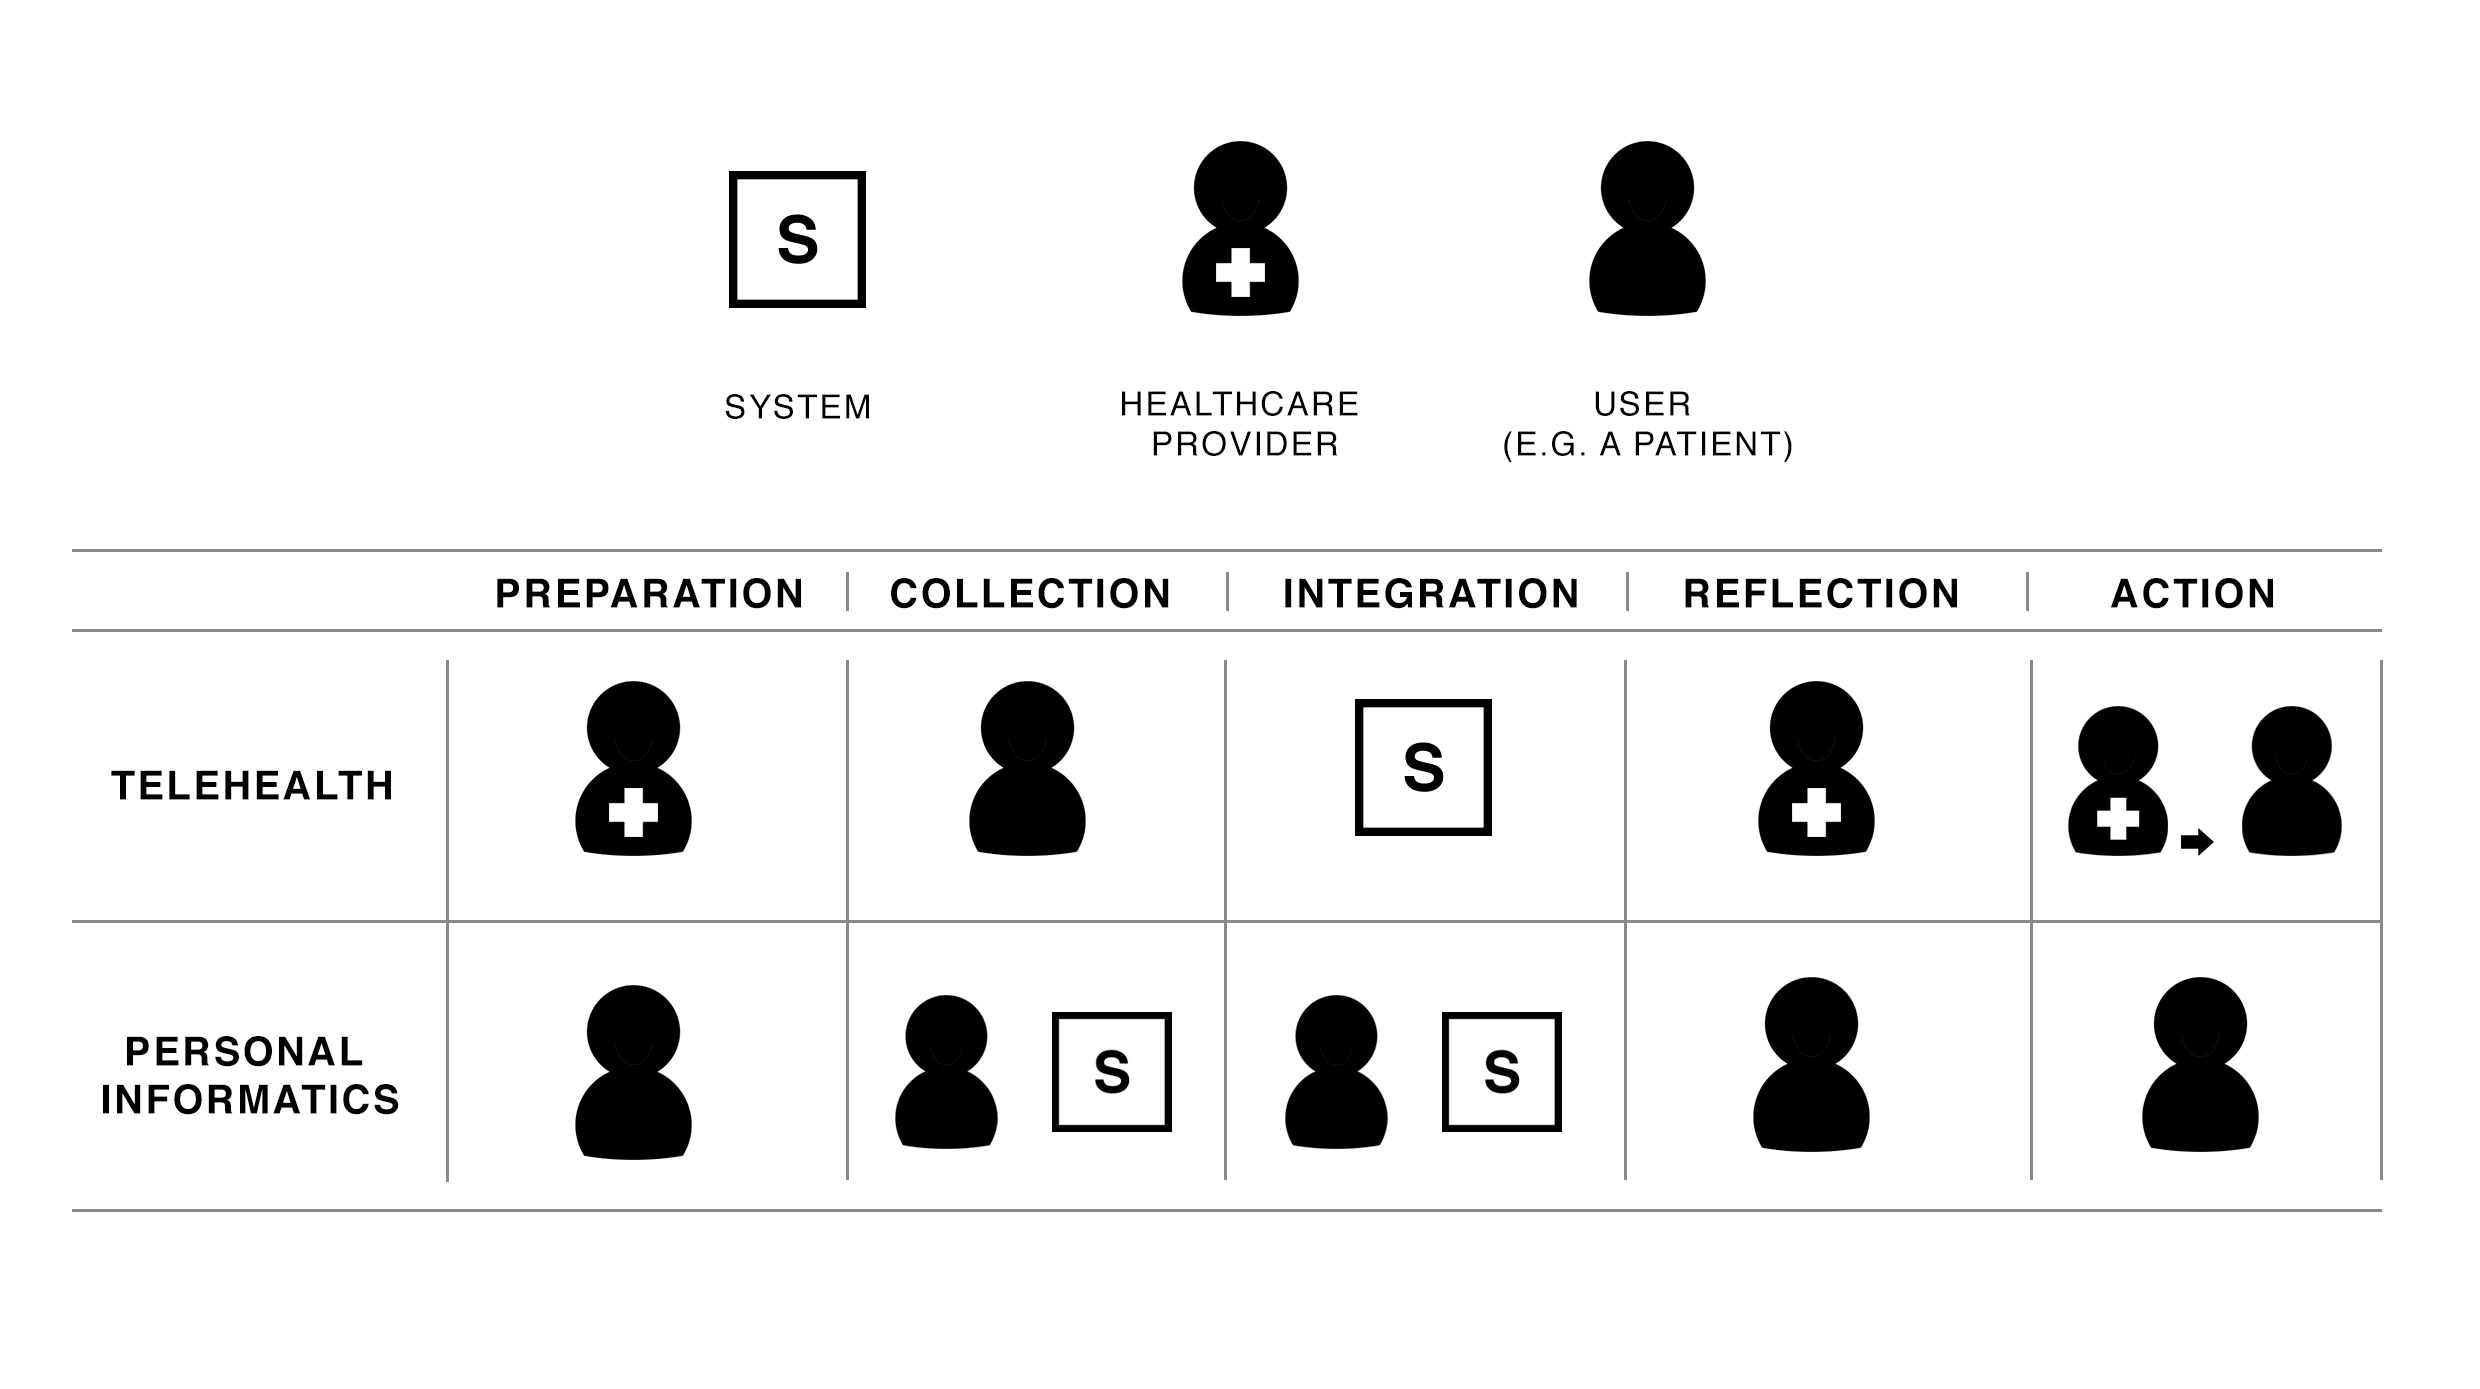
\includegraphics[width=0.9\columnwidth]{img/StakeholdersModel}
\caption{Stakeholders model bla bla}
\label{fig:StakeholdersModel}
\end{figure}

In telehealth, healthcare providers mandate and predefine what symptoms, how often and with what tool patients should track (\textit{preparation}). Patients collect both objective numerical (e.g. oxygen saturation measures) and subjective binary data (e.g. yes/no answers to whether dyspnea has increased more than usual) (\textit{collection}). The system integrates the data and based on predefined individual “normal ranges” flags data for follow-ups (\textit{integration}). Trained nurses or physicians review the self-tracked data (\textit{reflection}) in telehealth and if needed contact and advise the patient on potential initiation of treatment (\textit{action}) \cite{piloting, pedone}. 

Epstein et al. found that \textit{collection}, \textit{integration} and \textit{reflection} are ongoing processes that can occur simultaneously and integrated \textit{lapsing} (e.g. due to an oversight, holidays, injuries or when life habits change) and \textit{resuming} into their \textit{Lived Informatics Model} \cite{Epstein2015, Rooksby2014}. 

Rivera-Pelayo et al.\cite{Rivera} and Müller et al.\cite{Muller} discuss Personal Informatics in light of reflective learning theory (or learning by reflection) based on the work of Boud et al., who describe reflection as “those intellectual and affective activities in which individuals engage to explore their experiences in order to lead to new understandings and appreciations” \cite{Boud}. 

Rivera-Pelayo proposed a framework that shows three dimensions in which technology can support reflection: (1) Tracking, (2) Triggering and (3) Recalling and Revisiting. 
